\documentclass{article}
\usepackage{graphicx} % Required for inserting images





\documentclass[a4paper,12pt]{article}
\usepackage[utf8]{inputenc}
\usepackage{graphicx}
%  Русский язык
\usepackage{multirow}
\usepackage{wrapfig}
\usepackage[T2A]{fontenc}			% кодировка
\usepackage[utf8]{inputenc}			% кодировка исходного текста
\usepackage[english,russian]{babel}	% локализация и переносы

\usepackage{indentfirst} %Красная строка
\usepackage[a4paper,top=1.3cm,bottom=2cm,left=1.5cm,right=1.5cm,marginparwidth=0.5cm]{geometry}
\usepackage[usenames]{color}
\usepackage{colortbl}
\usepackage{csvsimple}
\usepackage{siunitx}
\usepackage{graphicx}
\graphicspath{ {images/} }
\usepackage{tikz}
\usepackage{pgfplots}

\usepackage{amsmath}
\usepackage{floatflt}
\usepackage[left=20mm, top=20mm, right=20mm, bottom=20mm, footskip=10mm]{geometry}

\usepackage{multicol}
\setlength{\columnsep}{2cm}

\usepackage{multicol}
\setlength{\columnsep}{2cm}
\usepackage{hyperref}


% Заметки
\usepackage{todonotes}

% Математика
\usepackage{amsmath,amsfonts,amssymb,amsthm,mathtools} 
\usepackage{hyperref}

\renewcommand{\AA}{\ensuremath{\mathring{A}}}

\begin{document}
\def\figurename{Рисунок}
\begin{titlepage}
\begin{center}
    {\large МОСКОВСКИЙ ФИЗИКО-ТЕХНИЧЕСКИЙ ИНСТИТУТ (НАЦИОНАЛЬНЫЙ ИССЛЕДОВАТЕЛЬСКИЙ УНИВЕРСИТЕТ)}
\end{center}
\begin{center}
    {\largeФизтех-школа биологической и медицинской физики}
\end{center}

\vspace{1cm}
{\huge
\begin{center}
    {\bf Лабораторная работа по общей физике}\\
    \vspace{0.5cm}
    4.3.3 Исследование разрешающей способности микроскопа методом Аббе
\end{center}
}

\vspace{4cm}
\begin{flushright}
{\LARGE Выполнила студентка группы Б06-103:\\ Фитэль Алена \\}

\end{flushright}
\vspace{9cm}
\begin{center}
    Долгопрудный, 2023 г.
\end{center}
\end{titlepage}
\newpage
\section{Введение}


\textbf{Цель работы}: определение дифракционного предела разрешения объектива микроскопа.

\textbf{В работе используются}: лазер; кассета с набором сеток разного периода; щель с микрометрическим винтом; оптический стол с набором рейтеров и крепёжных винтов; экран; линейка.


\section{Теоретические сведения}
Для иммерсионного микроскопа разрешающая способность объектива при некогерентном освещении
\begin{equation}
\ell_{min} \approx \dfrac{0.61\lambda}{\sin u},
\end{equation}
где $u$ -- апертурный угол объектива микроскопа (угол между оптической осью и лучом, направленным из центра объекта в край линзы).

Метод Аббе для оценки разрешающей способности состоит в разделении хода лучей на две части: сначала рассматривается картина в задней фокальной плоскости $F$ объектива -- она называется первичным изображением. Это первичное изображение рассматривается как источник волн, создающий вторичное изображение в плоскости $P_2$, сопряжённой плоскости предмета.\\
Первичное изображение есть картина дифракции Фраунгофера (на дифракционной решётке), если её период $d$, то для направления максимальной интенсивности $\varphi_m$
\begin{equation}
d \sin \varphi_m = m\lambda.
\end{equation}
При этом проходят пучки только с $\varphi_m < u$. Можно условием разрешения считать, что $u > \varphi_1$, иначе говоря
$$
\sin u \geq \lambda/d.
$$
или
\begin{equation}
\label{equ:allow}
d \geq \dfrac{\lambda}{\sin u} \approx \dfrac{\lambda}{D/2f},
\end{equation}
где $D$ -- диаметр линзы, $f$ -- фокусное расстояние.\\
Сетку можно рассматривать как две перпендикулярные друг другу решетки, для максимумов которых выполняется соотношение
\begin{equation}
\begin{array}{c c}
d\sin \varphi_x = m_x \lambda, & d\sin \varphi_y = m_y \lambda. \\
\end{array}
\end{equation}

\section{Экспериментальная установка}
\begin{figure}[h]
	\centering
	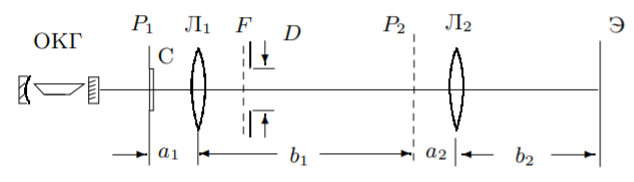
\includegraphics[scale=0.7]{stand.png}
	\caption{Схема установки}
	\label{fig:stand}
\end{figure}
Схема установки приведена на Рис. \ref{fig:stand}. Предметом $P_1$ служат сетки в кассете $C$. Линза $\text{Л}_1$ длиннофокусная, а $\text{Л}_2$ короткофокусная. В $F$ устанавливаются диафрагмы $D$, с помощью сеток с разными $d$ и щелевой диафрагмы можно проверить соотношение (\ref{equ:allow}). Период сеток может быть измерен либо по расстоянию между дифракционными максимумами на экране, либо по увеличенному с помощью микроскопа изображению. Пространственную фильтрацию (получение наклонного изображение решётки) можно получить с помощью подбора угла наклона и ширины вспомогательной щели.

\section{Обработка результатов}

\end{document}
